\subsection{Construcci\'on del modelo}

Sean $r_e, r_i \in \mathcal{R}$ el radio exterior de la pared del horno y el radio interno respectivamente. Llamaremos $T(r,\theta)$ a la temperatura en el punto dado por las coordenadas polares $(r,\theta)$, siendo $r$ el radio y $\theta$ el \'angulo polar de dicho punto. En estado estacionario, esta temperatura satisface la ecuaci\'on de calor:

~

\begin{equation}
 \frac{\partial T(r,\theta)}{\partial r^2} + \frac{1}{r} \frac{\partial T(r,\theta)}{\partial r} + \frac{1}{r^2} \frac{\partial^2T(r,\theta)}{\partial\theta^2} = 0
\end{equation}

~

Si llamamos $T_i \in \mathcal{R}$ a la temperatura en el interior del horno y $T_e:[0,2\pi] \rightarrow \mathcal{R}$ a la funci\'on de temperatura en el borde exterior del horno (correspondiente a los sensores) tendremos que $T(r,\theta) = T_i$ para todo punto $(r,\theta)$ con $r \leq r_i$ y que $T(r_e, \theta) = T_e(\theta)$ para todo punto $(r_e, \theta)$.

~

Para construir nuestro modelo y lograr una resoluci\'on computacional comenzaremos con una discretizaci\'on del dominio del problema a resolver, ya que el mismo en la vida real tiene infinitos radios y \'angulos. Consideraremos las siguientes particiones:

\begin{itemize}
 \item $0 = \theta_0 < \theta_1 < ... < \theta_n = 2 \pi$ en $n$ \textbf{\'angulos} discretos con $\theta_k - \theta_{k-1} = 2\pi/n = \Delta\theta$ para $k = 1,...,n$.
 \item $r_i = r_0 < r_1 < ... < r_m = r_e$ en $m$ \textbf{radios} discretos con $r_j - r_{j-1} = (r_i - r_e)/(m-1) = \Delta r$ para $j=1,...,m$.
\end{itemize}

Es importante remarcar que la discretizaci\'on de los \'angulos esta en limitada por la cantidad de sensores que tendremos en el horno real, no pudiendo superar a la cantidad de los mismos ya que ser\'an nuestros datos de entrada.

Una vez discretizados los valores de las coordenadas polares el problema ahora consiste en determinar el valor de la funci\'on $T$ en los puntos $(r_j, \theta_k)$. Llamemos $t_{jk} = T(r_j, \theta_k)$ al valor de la funci\'on $T$ en el punto $(r_j, \theta_k)$, cuyos valores son desconocidos. Aproximaremos las derivadas de la ecuaci\'on (1) de la siguiente manera:

~

\begin{equation}
 \frac{\partial T(r,\theta)}{\partial r^2}(r_j,\theta_k) \cong 
 \frac{t_{j-1,k}-2t_{j,k}+t_{j+1,k}}{(\Delta r)^2}
\end{equation}

\begin{equation}
 \frac{\partial T(r,\theta)}{\partial r}(r_j,\theta_k) \cong
 \frac{t_{j,k}-t_{j-1,k}}{\Delta r} 
\end{equation}

\begin{equation}
 \frac{\partial^2T(r,\theta)}{\partial\theta^2}(r_j,\theta_k) \cong
 \frac{t_{j,k-1}-2t_{j,k}+t_{j,k+1}}{(\Delta \theta)^2}
\end{equation}

~

~

Si reemplazamos las aproximaciones (2), (3) y (4) en (1) obtendremos:

~

\begin{equation}
 \frac{t_{j-1,k}-2t_{j,k}+t_{j+1,k}}{(\Delta r)^2} 
 + \frac{t_{j,k}-t_{j-1,k}}{r(\Delta r)} 
 + \frac{t_{j,k-1}-2t_{j,k}+t_{j,k+1}}{r^2(\Delta \theta)^2}
 = 0
\end{equation}

~

~

Para cada punto $(r_j,\theta_k)$, lo que nos deja con un sistema de ecuaciones lineales que modela el problema discretizado.

\newpage
\subsection{Idea de resoluci\'on}

La idea es resolver el sistema de ecuaciones en un primer lugar represent\'andolo en matrices y luego utilizando eliminaci\'on Gaussiana y factorizaci\'on LU para resolver el mismo. El sistema quedar\'a de la forma $At = b$ siendo $t$ y $b$ vectores columna  en donde $A$ contendr\'a a los coeficientes de la ecuaci\'on de calor (5), $b$ contendr\'a los datos para resolver el sistema y $t$ contendr\'a cada punto interno del horno correspondiente con la discretizaci\'on.

~

Los vectores columna $t$ y $b$ tendr\'an ambos dimensi\'on $nm$. La estructura de $t$ estar\'a conformada por los valores $t_{1,1}, t_{1,2}, ..., t_{1,n}, t_{2,1} ..., t_{m,n}$ dispuestos en forma de columna. Por otro lado, el vector $b$ tendr\'a el valor $1500$ en las primeras $n$ posiciones (correspondientes al radio interno del horno), ceros en las siguientes $m(n-2)$ posiciones y los valores correspondientes a $T_e(\theta_1), T_e(\theta_2), ..., T_e(\theta_n)$ en las \'ultimas $n$ posiciones (correspondientes a los valores de los sensores).

~


 \begin{equation*}
\left( \begin{array}{ccccccc}
1 & 0 & 0 & 0 & 0 & \dots & 0\\
0 & 1 & 0 & 0 & 0 & \dots & 0\\
\vdots & & \ddots & & & & \vdots\\
0  & \dots & 0 & 1 & 0 & \dots  & 0\\

  & \dots &  & t_{i,j-1} & t_{i,j} & \dots &\\

\vdots & & & \vdots & & & \vdots\\
0  & \dots & & 0 & & \dots  & 1\\
\end{array} \right)
\left( \begin{array}{c}
t_{1,1} \\
t_{1,2} \\
\vdots \\
t_{1,n} \\
t_{2,1} \\
\vdots \\
t_{m,n} \\ \end{array} \right)
= \left( \begin{array}{c}
1500 \\
1500 \\
\vdots \\
1500\\
0\\
\vdots\\
T_e(\theta_n)\end{array} \right)
\end{equation*}

~

~

La matriz $A$ por otro lado ser\'a cuadrada de tama\~no $nm$ en cada dimensi\'on. Las primeras $n$ filas ser\'an una identidad que se corresponder\'a con las temperaturas en el radio interno, que como son dato las conocemos. Las siguientes $m(n-2)$ filas corresponder\'an a las ecuaciones de calor por cada punto interno de la discretizaci\'on. Cada ecuaci\'on tendr\'a $nm$ t\'erminos (aunque la mayor\'ia de ellos acompa\~nados por un coeficiente nulo) por lo que la matriz tendr\'a $nm$ columnas. Finalmente en las ultimas $n$ filas de la matriz se encontrar\'a la identidad que se corresponder\'a con las temperaturas externas, es decir aquellas registradas por los sensores.

~

Ahora solamente nos falta saber como llenar $A$. Si hacemos un manejo algebraico sobre la ecuaci\'on (5) juntando los elementos iguales nos queda que:

\begin{equation*} \implies
 \frac{t_{j-1,k}}{(\Delta r)^2}
 -\frac{2t_{j,k}}{(\Delta r)^2}
 +\frac{t_{j+1,k}}{(\Delta r)^2}
 +\frac{t_{j,k}}{r(\Delta r)}
 -\frac{t_{j-1,k}}{r(\Delta r)}
 +\frac{t_{j,k-1}}{r^2(\Delta \theta)^2}
 -\frac{2t_{j,k}}{r^2(\Delta \theta)^2}
 +\frac{t_{j,k+1}}{r^2(\Delta \theta)^2} = 0
\end{equation*}

\begin{equation*} \implies
 \frac{t_{j,k}}{r(\Delta r)}
 -\frac{2t_{j,k}}{(\Delta r)^2}
 -\frac{2t_{j,k}}{r^2(\Delta \theta)^2}
 +\frac{t_{j-1,k}}{(\Delta r)^2}
 -\frac{t_{j-1,k}}{r(\Delta r)}
 +\frac{t_{j+1,k}}{(\Delta r)^2}
 +\frac{t_{j,k-1}}{r^2(\Delta \theta)^2}
 +\frac{t_{j,k+1}}{r^2(\Delta \theta)^2} = 0
\end{equation*}

~

~

Es decir que me queda para la ecuaci\'on correspondiente a cada $t_{j,k}$:

\begin{figure}[!htb]
\centering
\minipage{0.5\textwidth}
  \begin{equation}
  c_1 = c_{j,k} = \frac{1}{r\Delta r}-\frac{2}{(\Delta r)^2}-\frac{2}{(r\Delta \theta)^2}
  \end{equation}

  \begin{equation}
  c_2 = c_{j-1,k} = \frac{1}{(\Delta r)^2}-\frac{1}{r\Delta r}
  \end{equation}

  \begin{equation}
  c_3 = c_{j+1,k} = \frac{1}{(\Delta r)^2}
  \end{equation}

  \begin{equation}
  c_4 = c_{j,k-1} = c_{j,k+1} = \frac{1}{(r\Delta \theta)^2}
  \end{equation}
\endminipage\hfill
\minipage{0.5\textwidth}
  
  $$r = r_i + (j-1)(\Delta r)$$
  
  $$\Delta \theta = 2\pi/n$$
  
  $$\Delta r = (r_i-r_e)/(m-1)$$
  
\endminipage\hfill
\end{figure}

Finalmente para llenar $A$ la inicializaremos en cero y luego nos moveremos por la diagonal. Si estamos en alguna de las dos \'areas de identidad, es decir las primeras o \'ultimas $n$ filas, pondremos un $1$. De lo contrario asignaremos el valor correspondiente a $c_{j,k}$ para el $j$ y $k$ apropiados y los otros $4$ valores en las posiciones correspondientes. En los casos en modificamos $j$ nos moveremos $n$ columnas hacia la izquierda si restamos y hacia la derecha si sumamos. En los casos en los que $k+1$ o $k-1$ se salgan fuera del rango $[1,n]$ le aplicaremos m\'odulo $n$, moviendonos as\'i $n-1$ columnas hacia la izquierda o derecha respectivamente.

%TODO: Imagen explicativa de esto ^^^

\newpage
\subsection{Algoritmos}

\begin{figure}[!htb]
\centering
\minipage{0.5\textwidth}
  \begin{algorithmic}[1]
  \Function{WithFifteenThetas}{$r_i$, $r_e$, $n$, $m$, $T_i$, $T_e$}
    \State $dr \leftarrow (r_e - r_i) / (m - 1)$
    \State $dt \leftarrow 2\pi/n$
    \State \textbf{Matrix} $b \in \mathcal{R}^{nm\times 1}, A\in \mathcal{R}^{nm\times nm}$
    \For{$i \in [1,nm]$}
      \State $b[i][1] \leftarrow T_i[i]$
      \State $b[nm-i][1] \leftarrow T_e[i]$
    \EndFor
    \State $j \leftarrow 1, k \leftarrow 1$
    \For{$i \in [1,nm]$}
      \If{$i \in [1,n] \vee i \in [(n-1)m,nm]$}
	\State $A[i][i] \leftarrow 1$
      \Else
	
	\State $A[i][i] \leftarrow c_1(j, r_i, dr, dt)$
	\State $A[i][i-n] \leftarrow c_2(j, r_i, dr, dt)$
	\State $A[i][i+n] \leftarrow c_3(j, r_i, dr, dt)$
	
	\If{$k=n$}
	  \State $A[i][i-n+1] \leftarrow c_4(j, r_i, dr, dt)$
	\Else
	  \State $A[i][i+1] \leftarrow c_4(j, r_i, dr, dt)$
	\EndIf
	
	\If{$k=1$}
	  \State $A[i][i+n-1] \leftarrow c_4(j, r_i, dr, dt)$
	\Else
	  \State $A[i][i-1] \leftarrow c_4(j, r_i, dr, dt)$
	\EndIf

	\State $k \leftarrow k+1$      
	\If{$k>n$}
	  \State $j \leftarrow j+1, k \leftarrow 1$
	\EndIf
	
      \EndIf
    \EndFor
    \State \Return $solve(A,b)$
  \EndFunction
  \end{algorithmic} 
  
  ~
  
  \begin{algorithmic}[1]
    \Function{BackSub}{\textbf{Matrix} $A$, \textbf{Matrix} $b$}
      \State \textbf{Matrix} $R \in \mathcal{R}^{cols(A)\times 1}$
      
      \For{$i \in [A.n, 1]$}
	 \If{$a_{i,i} \not= 0$}
	    \State $r_{i,1} \leftarrow (b_{i,1} - A[i] \times R) / a_{i,i}$
	 \EndIf
      \EndFor
      
      \State \Return $R$
    \EndFunction
  \end{algorithmic}   
  
  ~
  
  \begin{algorithmic}[1]
    \Function{ForwSub}{\textbf{Matrix} $A$, \textbf{Matrix} $b$}
      \State \textbf{Matrix} $R \in \mathcal{R}^{cols(A)\times 1}$
      
      \For{$i \in [1, A.n]$}
	 \If{$a_{i,i} \not= 0$}
	    \State $r_{i,1} \leftarrow (b_{i,1} - A[i] \times R) / a_{i,i}$
	 \EndIf
      \EndFor
      
      \State \Return $R$
    \EndFunction
  \end{algorithmic} 
  
\endminipage\hfill
\minipage{0.01\textwidth}
\endminipage\hfill
\minipage{0.49\textwidth}

\textbf{WithFifteenThetas} es la funci\'on principal encargada de la resoluci\'on de una instancia del problema. Consideramos con fines pr\'acticos que ya recibe los datos procesados del input por los par\'ametros de radio interno ($r_i$), radio externo ($r_e$), cantidad de \'angulos ($n$), cantidad de radios ($m$), un vector de temperaturas internas ($T_i$) y un vector de temperaturas externas ($T_e$).  

~

Entre las lineas 2 a 9 se inicializan los valores de $\Delta r$ ($dr$) y $\Delta \theta$ ($dt$) y se carga el vector columna $b$ con los valores provenientes de $T_i$ y $T_e$, quedando en los $n$ primeros lugares los valores de $T_i$ y en los $n$ \'ultimos los valores de $T_e$. En la linea 9 se puede observar la inicializaci\'on de los contadores $j$ y $k$. Entre las lineas 10 a 32 tenemos el bucle responsable de llenar la matriz $A$. Como explicamos en la secci\'on anterior, la idea es moverse por la diagonal y si se encuentra en un \'area identidad asignar un $1$ (lineas 11 y 12). De lo contrario, asignaremos el coeficiente $c_1$ a la posici\'on de la diagonal y $c_2$, $c_3$ y $c_4$ a las columnas correspondientes de esa misma fila. Los coeficientes son calculados como se los muestra en las formulas (6), (7), (8) y (9). 

Finalmente en la linea 33 se llama a la funci\'on solve que resuelve el sistema lineal. En nuestra implementaci\'on en ese momento se llama a solveGE (resoluci\'on por eliminaci\'on Gaussiana) o solveLU (resoluci\'on por factorizaci\'on LU) dependiendo del modo en el que se este usando el programa. Para simplicidad del pseudoc\'odigo decidimos dejar fuera dicho detalle ya que pertenece mas a la implementaci\'on. El llenado de la matriz $A$ tiene una complejidad de $\mathcal{O}(nm)$.

~

\textbf{BackSub} (backSubstitution) y \textbf{ForwSub} (forwardSubstitution) realizan la resoluci\'on de un sistema con una matriz $A$ diagonal superior y diagonal inferior respectivamente. En \textbf{BackSub} en la linea 2 se inicializa con ceros el vector columna en donde se devolver\'a el resultado. Luego entre las lineas 3 a 7, se procede a iterar movi\'endose por la diagonal. Si se encuentra un cero se saltea esa fila (linea 4), ya que de haberse encontrado toda la fila es cero. De lo contrario en la linea 5 se multiplica la fila $i$ de $A$ ($A[i]$) por el vector resultado ($R$), se lo resta a el dato correspondiente a esa ecuaci\'on y se lo divide por el coeficiente de la inc\'ognita que se quiere despejar. 

Si nos detenemos a observar esta \'ultima operaci\'on, podremos ver que lo que se esta haciendo es encontrar el valor de $x_i$ despejando la ecuaci\'on $a_{i,i}x_i + A[i] \times R = b_{i,1}$ en donde $A[i] \times R$ es la suma de los $x_i$ conocidos por sus constantes. En la linea 8 el algoritmo devuelve el resultado, que una vez terminadas las iteraciones contendr\'a los valores que resuelven el sistema ordenados de forma $x_1, x_2, ..., x_{cols(A)}$. \textbf{BackSub} tiene una complejidad de $\mathcal{O}(n^2)$.

~

\textbf{ForwSub} tiene un comportamiento isomorfo a \textbf{BackSub}, la \'unica diferencia es que comienza despejando la primera ecuaci\'on en lugar de la \'ultima y sigue desde all\'i hasta la \'ultima. 


\endminipage\hfill
\end{figure}

\newpage
\begin{figure}[!htb]
\centering
\minipage{0.5\textwidth}
  
  \begin{algorithmic}[1]
    \Function{SolveGE}{\textbf{Matrix} $A$, \textbf{Matrix} $b$}    
      \For{$i \in [1, A.m)$}
	\For{$z \in [i+1, A.m]$}
	   \State $A[z] \leftarrow A[z] - (a_{z,i}/a_{i,i})\cdot A[i]$
	   \State $b[z] \leftarrow (-a_{z,i}/a_{i,i})\cdot b[i]$
	\EndFor
      \EndFor
      \State \Return $backSub(A,b)$
    \EndFunction
  \end{algorithmic} 
  
  ~
  
  ~
  
  \begin{algorithmic}[1] 
    \Function{SolveLU}{\textbf{Matrix} $A$, \textbf{Matrix} $b$}
      \State \textbf{Matrix} $LU \leftarrow decompLU(A)$
      \State \textbf{Matrix} $y \leftarrow forwSub(LU.first,b)$
      \State \Return $backSub(LU.second,y)$
    \EndFunction
  \end{algorithmic}
  
  ~
  
  ~
  
  \begin{algorithmic}[1]
    \Function{DecompLU}{\textbf{Matrix} $A$}
      \State \textbf{Matrix} $L \in \mathcal{R}^{nm\times nm}$
      \State \textbf{Matrix} $U \in \mathcal{R}^{nm\times nm}$
      
      \For{$i \in [1, A.m)$}
	\For{$z \in [i+1, A.m]$}
	    \State $l_{z,i} \leftarrow a_{z,i}/a_{i,i}$
	    \State $U[z] \leftarrow A[z] - (a_{z,i}/a_{i,i})\cdot A[i]$
	\EndFor
	\State $l_{i,i} \leftarrow 1$
      \EndFor
      \State $L[A.m][A.m] \leftarrow 1$
      
      \State \Return <$L,U$>
    \EndFunction
  \end{algorithmic} 
  
\endminipage\hfill
\minipage{0.01\textwidth}
\endminipage\hfill
\minipage{0.49\textwidth}

\textbf{SolveGe} (solverGaussianElimination) utiliza la eliminaci\'on Gausseana para diagonalizar superiormente el sistema y luego lo resuelve utilizando backSubstitution. En nuestro algoritmo, en las lineas 2 y 3 a 6 y 7 se pueden observar los for principales del mismo. El primer for, cuyo contador es $i$, se encarga de apuntar a la fila que se esta usando para conseguir ceros en las dem\'as. El segundo for, a quien el contador $j$ le pertenece, se encarga de iterar por las filas inferiores a la fila $i$. 

En cada iteraci\'on se le resta a la fila $z$ un m\'ultiplo de la fila $i$, de forma tal que se origine un cero en la posici\'on $(z,i)$ (linea 4). En la linea 5 se repite dicha operaci\'on con el vector columna $b$, de forma tal de conservar la concordancia con el sistema original. Una vez terminada la iteraci\'on completa del segundo for, los \'unicos lugares en donde habr\'an valores distintos de cero en la columna $i$, ser\'a en arriba de la diagonal. Finalmente con la matriz diagonalizada superiormente se utiliza el algoritmo de backSub para devolver una resoluci\'on al sistema. La complejidad de la eliminaci\'on Gausseana es de $\mathcal{O}(n^3 + n^2) \subseteq \mathcal{O}(n^3)$.

~

\textbf{SolveLU} utiliza la factorizaci\'on LU para separar el sistema original en dos sistemas que juntos son equivalentes al original. Al separarlos, una de de las matrices queda diagonalizada de forma inferior (L) y la otra de forma superior (U). Luego se puede resolver el sistema utilizando forwardSubstitution para el sistema inferior y backSubstitution para el sistema superior. La ventaja de este m\'etodo es que el vector columna $b$ no es modificado en la diagonalizaci\'on y por lo tanto podremos guardarnos las matrices $L$ y $U$ para resolver sistemas con un $b$ distinto ahorr\'andonos el costo de la diagonalizaci\'on.

\endminipage\hfill
\end{figure}

La funci\'on \textbf{DecompLU} sirve para descomponer una matriz $A$ en dos matrices $L$ y $U$ de forma tal que se cumpla que $L\cdot U = A$. Es b\'asicamente una eliminaci\'on Gausseana que guarda en la matriz $L$ los coeficientes que se van utilizando en cada paso (linea 6), adem\'as de colocarle en la diagonal todos unos (linea 9 y 11). Una vez terminada la diagonalizaci\'on devuelve una tupla con ambas matrices. 


\begin{SCfigure}[1][ht!]
\sidecaptionvpos{figure}{t}
  \caption{ Realizando un spy en Matlab luego de llenar la matriz con el algoritmo propuesto anteriormente pudimos visualizar que su llenado era correcto. En la imagen se pueden observar aproximadamente las primeras 70 filas y columnas de la matriz, en las que se aprecia la identidad en las primeras filas y luego la forma caracter\'istica que deber\'ia tener por las coordenadas polares involucradas y sus saltos de columnas al restarse o sumarse a alguna de ellas.\newline\newline\newline\newline\newline\newline}
  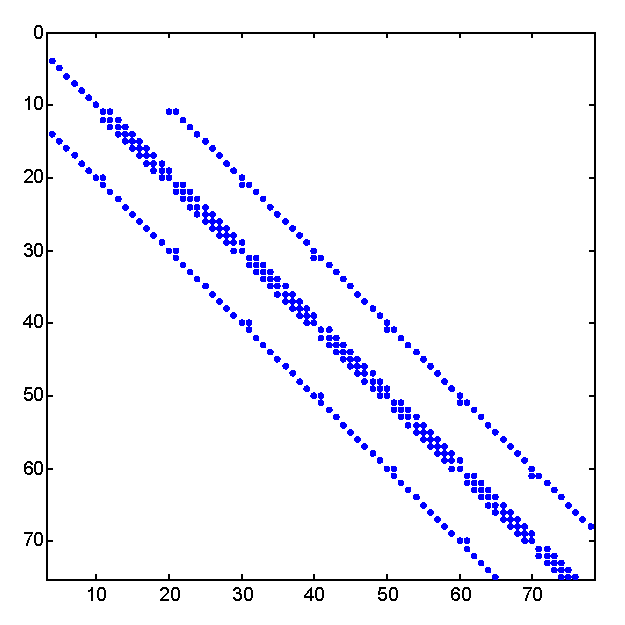
\includegraphics[width=0.4\textwidth]{figures/spy.pdf}
  \label{compbench-glu}
\end{SCfigure}

\newpage

En nuestra implementaci\'on este algoritmo funciona modificando solamente $A$ con el objetivo de ahorrar memoria. Esto se logra eliminando las lineas 11 y 9, haciendo las asignaciones a $A$ en vez de a $L$ y $U$ en las lineas 6 y 7 y devolviendo $A$ en vez de la tupla. Obviamente esta \'ultima modificaci\'on repercute tambi\'en en la funci\'on \textbf{SolveLU}, en la cual hacemos modificaciones en los algoritmos de \textbf{ForwSub} y \textbf{BackSub} para que solamente se muevan por ciertos \'indices de $A$ en cada caso, a forma de calcular correctamente la resoluci\'on de cada sistema sin la necesidad de utilizar dos matrices distintas. El motivo por el cual presentamos esta versi\'on mas b\'asica es porque es mas elegante y f\'acil de entender que su versi\'on optimizada.

~

La complejidad de \textbf{DecompLU} es de $\mathcal{O}(n^3)$, lo que desemboca en una complejidad de $\mathcal{O}(n^3 + 2n^2) \subseteq \mathcal{O}(n^3)$ para \textbf{SolveLU}. Sin embargo, es importante remarcar que si hacemos resoluciones del mismo sistema con la factorizaci\'on LU solamente deberemos resolver los sistemas diagonalizados, por lo que el costo de \textbf{SolveLU} se reduce a $\mathcal{O}(2n^2) \subseteq \mathcal{O}(n^2)$ para las resoluciones sucesivas a la primera. Finalmente podemos ver que \textbf{WithFifteenThetas} tiene una complejidad total de $\mathcal{O}(nm + (nm)^3) \subseteq \mathcal{O}((nm)^3)$ con \textbf{SolveGE} y con la primera resoluci\'on de \textbf{SolveLU}. Sin embargo, las sucesivas resoluciones con \textbf{SolveLU} del mismo sistema tienen una complejidad de $\mathcal{O}((nm)^2)$.

\begin{figure}[!htb]
\centering
\minipage{0.5\textwidth}

\begin{algorithmic}[1]
    \Function{getIsoterm}{\textbf{Vector} $T$, $n$, $m$, $iso$}
      \State \textbf{Vector} $res \in \mathcal{R}^{n}$

      \For{$k \in [0, n)$}
	  \State{\textbf{int} best $\leftarrow$ 0}

	  \For{$j \in [0, m)$}
	      \State {best $\leftarrow$ j}
	      \If{$T[j * n + k][0] < iso$}
		  \State \textbf{break}
	      \EndIf
	  \EndFor

	  \State{\textbf{double} dr $\leftarrow$ $\frac{r_e - r_i}{m - 1}$}

	  \If{best $\geq m $}
	      \State{$res_{k} \leftarrow r_e$}
	      \State{continue}
	  \EndIf

	  \State{$r_2 \leftarrow best$}
	  \State{$r_1 \leftarrow best - 1$}

	  \State{$t_1 = T[r_1 * n + k][0]$}
	  \State{$t_2 = T[r_2 * n + k][0]$}
	  \State{$res_{k} \leftarrow (isovalue - t_1) * \frac{r_2 - r_1}{t_2 - t_1} + r_1$}

	  \State{$res_{k} \leftarrow res_{k} * dr$}
	  \State{$res_{k} \leftarrow res_{k} + r_i$}
    \EndFor
    
    \State \Return $res$
  \EndFunction
\end{algorithmic}   

\endminipage\hfill
\minipage{0.01\textwidth}
\endminipage\hfill
\minipage{0.49\textwidth}

Finalmente, \textbf{getIsoterm} es la función que calcula la curva isoterma. Toma como argumentos la matriz de temperaturas, la cantidad de \'angulos y radios, y el valor de temperatura buscado. Luego devuelve un vector con los radios por los que pasa la curva para cada \'angulo $\theta$.
En la linea 2 se encuentra el ciclo principal, que se encarga de recorrer los \'angulos, para poder calcular el radio por el cual pasa la isoterma  en cada \'angulo por separado.  El ciclo de la linea 5 se encarga de recorrer radialmente en dicho \'angulo hasta que la temperatura sea menor que la isoterma buscada (aquí se asume que avanzando radialmente, las temperaturas solo pueden disminuir), con lo cual el radio buscado esta entre este radio, el j-ésimo y el anterior.  Estos valores luego son guardados en la variable '$r_2$' y '$r_1$', y sus temperaturas en $t_2$ y $t_1$ respectivamente.
Para interpolar se usa la inversa de una recta, que pasa por los puntos ($r_1$, $t_1$) y ($r2$, $t2$). Dicha recta, dentro de su dominio $[r_1,r_2]$, trabajar\'ia como una función interpoladora que devuelve la temperatura, dado un radio. Pero al usar su inversa, sucede que al dar el valor de una temperatura (que en este caso sera siempre el de la isoterma), devuelve el radio del que provino. Este valor es asignado a $res_{k}$ y luego multiplicado por delta r y adicionado a $r_{i}$ para que represente el valor del radio real.
Aquí termina el ciclo principal y se realiza el calculo nuevamente para el siguiente \'angulo, hasta recorrerlos todos. La función retorna el vector de radios de la isoterma por el vector '$res$'.

\endminipage\hfill
\end{figure}


